%\chapter{Measurement of the electroweak diboson production with dijet in semileptonic final states}
\chapter{Signal and Background processes}
\label{chap:sigbkg}
In the following chapters, the measurement of an electroweak (EW) diboson (VV) production in association with a high-mass dijet system (jj) in the semileptonic final states is studied.
This process is sensitive to the VBS process described in section~\ref{sec:VBS}.
\section{Feature of the process}
EW VV jj process is experimentary identified with the existence of two bosons ( VV = WW, ZZ, or WZ ) with two jets in opposite hemisphere with a large dijet invariant mass.
The typical EW VV jj processes are shown in diagrams of figure~\ref{fig:feynmanEWVVjj}.
The VBS diagrams, which is physically most interested one is included as shown in the left of the figure~\ref{fig:feynmanEWVVjj}. The figure in the middle and the right represnet non-VBS EW and QCD VV jj production. EW non-VBS diagrams are also included in the signal process since they cannot be distinguished from VBS process for the gauge invariant conservation, while QCD non-VBS processes separated from the signal and considered as background.

\begin{figure}[H]
\begin{center}
 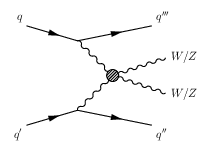
\includegraphics[width=0.3\textwidth,keepaspectratio]{figures/EWVVjj_a.png}
 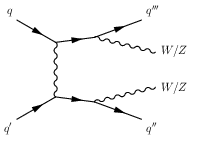
\includegraphics[width=0.3\textwidth,keepaspectratio]{figures/EWVVjj_b.png}
 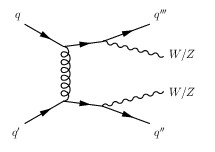
\includegraphics[width=0.3\textwidth,keepaspectratio]{figures/EWVVjj_c.png}

\caption[f]{
Feynman diagrams for EW VV jj signals. Each diagram shows VBS process (left), EW non-VBS process (middle), and QCD non-VBS process (right).
}
\label{fig:feynmanEWVVjj}
\end{center}
\end{figure}


%Theoretically, VBS processes shown in Fig~\ref{fig:feynmanVBS} cannot be distinguished from the other electroweak VV+jj proceses like diagrams shown in Fig~\ref{fig:feynmanEWKnonVBS2} and Fig~\ref{fig:feynmantZb}, for the gauge invariant conservation, hence they are generated altogether as electroweak (EW) VV+jj production.

This analysis focuses semileptonic final states, with one of the bosons decays leptonically, and the other hadronically. 
The schematic of the process is shown in Figure~\ref{fig:VBStopology}.

%The experimental characteristic of the VBS process is described by two vector bosons in the central region and the two jets which go forward in the opposite hemisphere.
%The kinematics of this process is illustrated in Figure~\ref{fig:VBStopology}.

\begin{figure}[H]
\begin{center}
 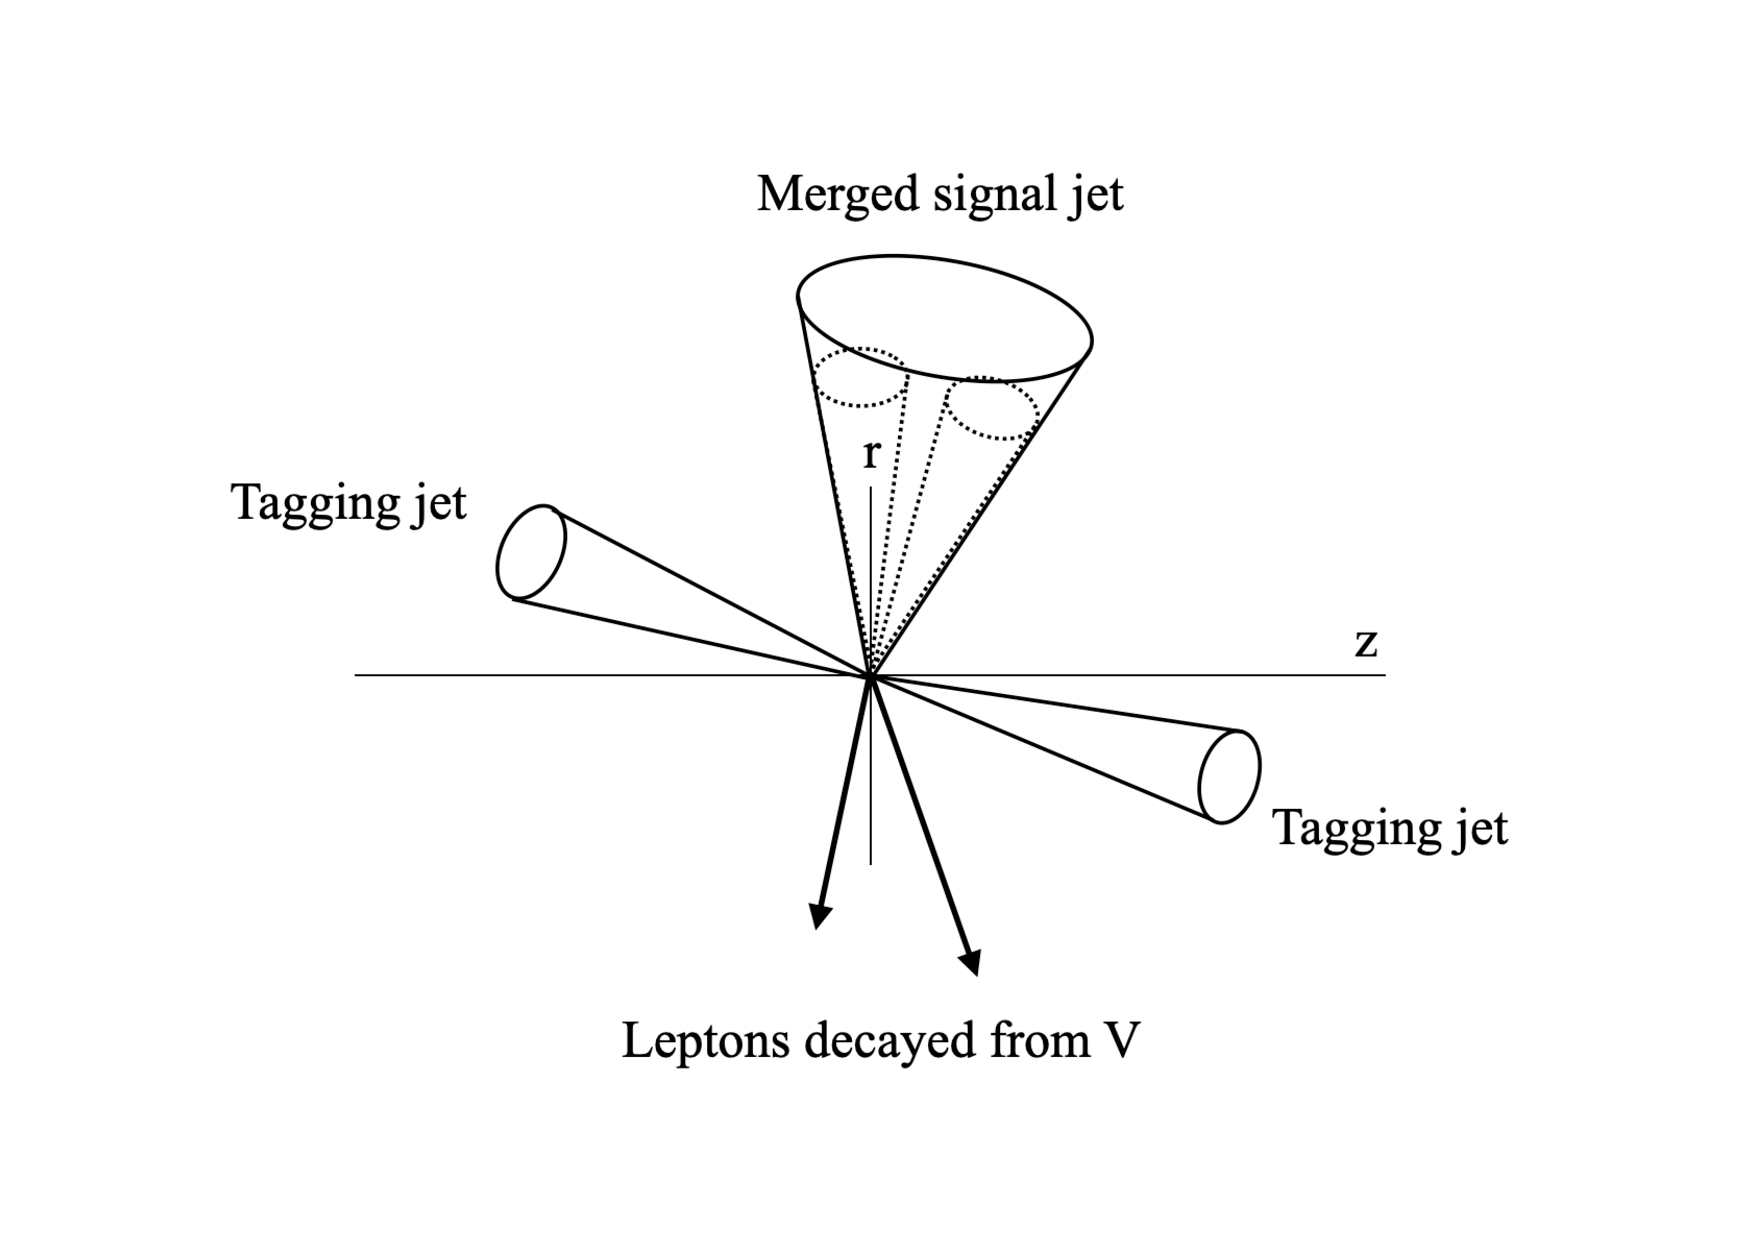
\includegraphics[width=0.50\textwidth,keepaspectratio]{figures/VBStopologyMerged}
 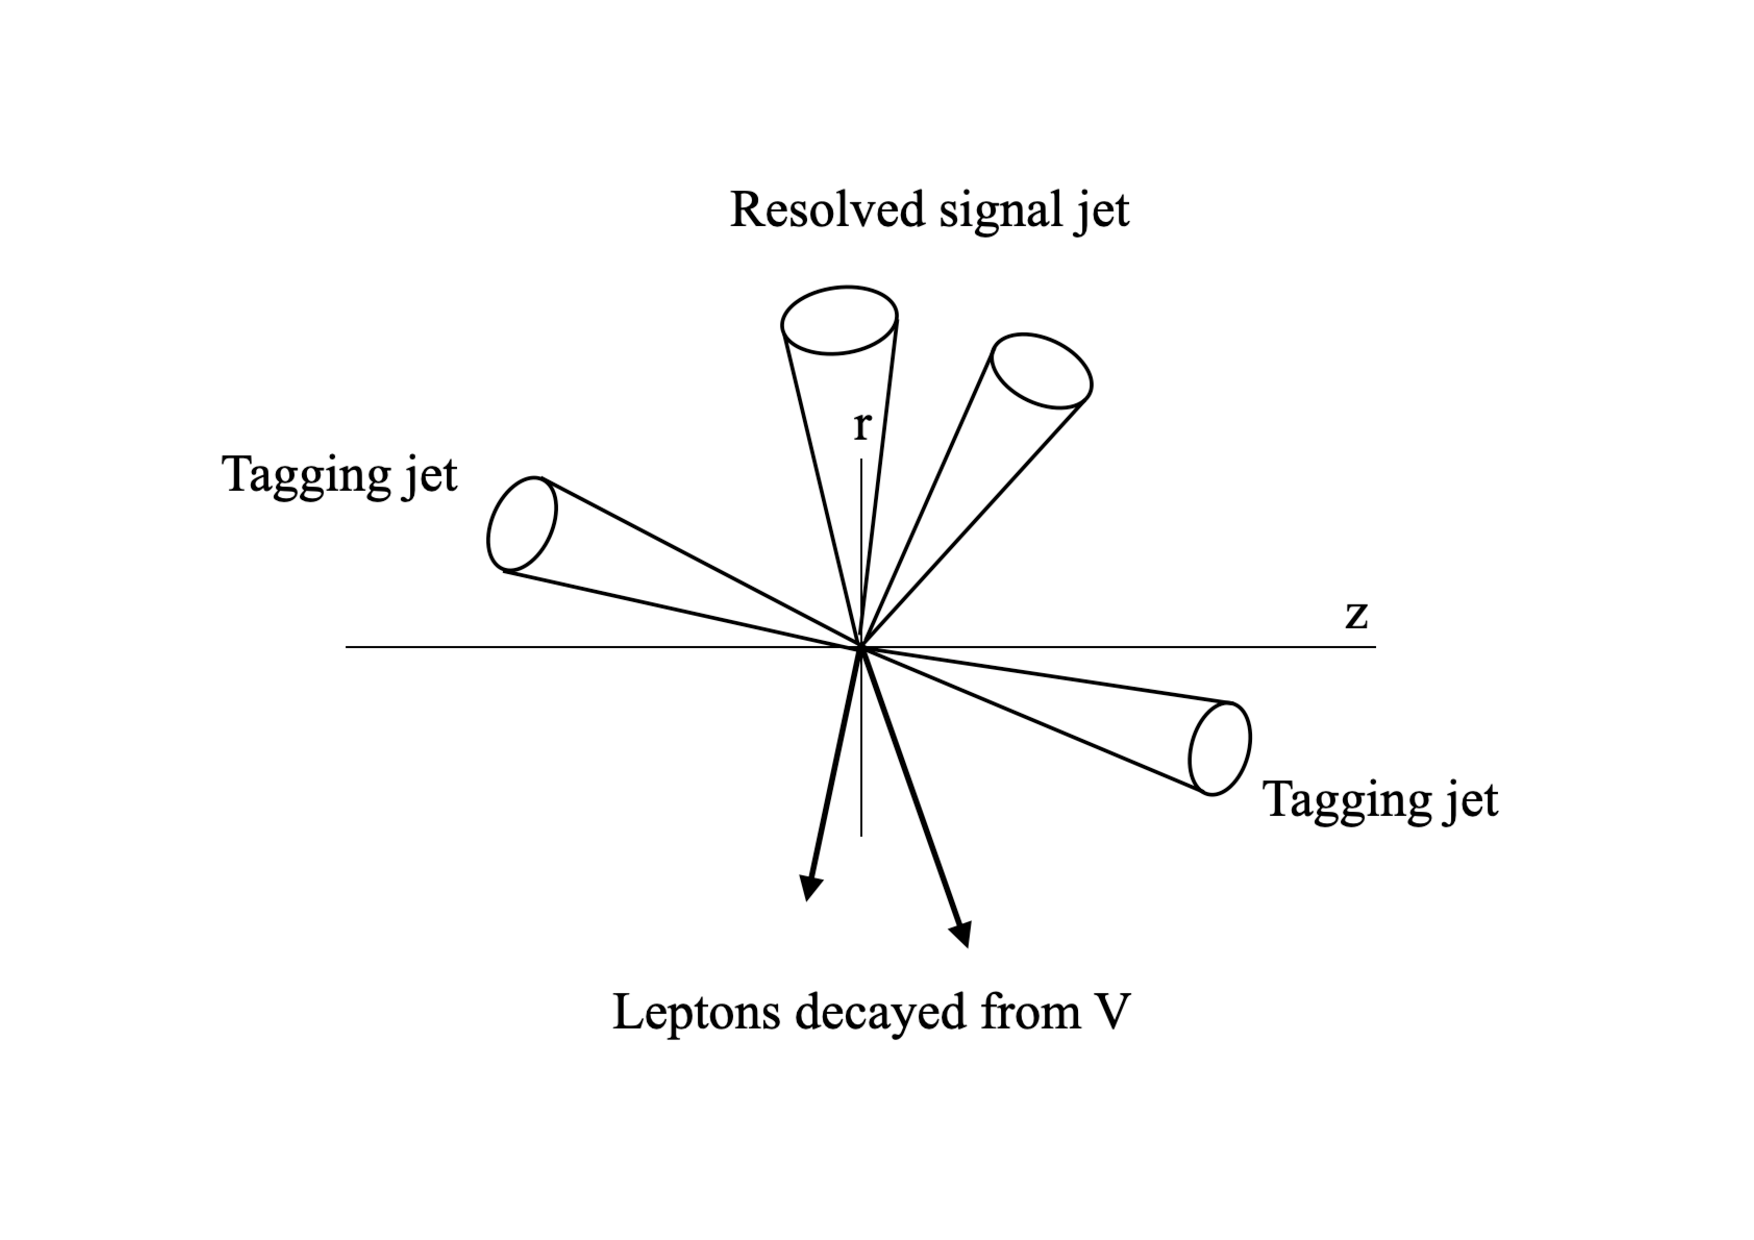
\includegraphics[width=0.45\textwidth,keepaspectratio]{figures/VBStopologyResolved}
\caption{
The schematic representation of a EW VV jj event. The hadronic day of the V is reconstructed as one large-R jet in the merged selection (left), or two small-R jets in resolved selection (right).
}
\label{fig:VBStopology}
\end{center}
\end{figure}

The analysis is spirited into three channels, due to the numbers of the charged leptons decayed from one of the bosons: 0-lepton, 1-lepton, 2-lepton. 
In 0-lepton channel, Z $\rightarrow \nu \nu$ is considered, experimentally reconstructed as missing transverse energy (MET). In 1-lepton channel one of the bosons decays as W $\rightarrow \nu l$ where we can find $l = e, \mu, \tau$ with MET. In 2-lepton channel Z $\rightarrow l l$ is required with $l = e, \mu$. 
In all three channels, the process requires hadronically decaying boson candidate, with 2 additional jets. These additional 2 jets are initially from the quarks from VBS production, referred as tagging jets. The hadronic decaying objects are reconstructed as a pair of small-R jets or as single large-R jet. The former case is called as resolved selection, and the latter as merged selection. More details about the objects in each category is shown in section~\ref{sec:object}.

The relevant background processes include W/Z + jets, single top (t) and tt-bar (t$\bar{\mathrm{t}}$) process, QCD diboson process, and QCD multijet process.
In 0-lepton channel, all of the background processes contribute significantly. In 1-lepton channel W + jets and the t$\bar{\mathrm{t}}$ process dominate, and in 2-lepton channel Z + jets process is the dominant process.

\section{Data and Monte Carlo Simulation}
\subsection{Data}
The data used in the analysis is collected from the ATLAS detector with pp collisions at a center of mass energy of 13 TeV during the full Run~2 during the years 2015 to 2018. The total integrated luminosity in this period is 139~fb$^{-1}$ with uncertainty of 1.7~\% \cite{DAPR-2010-01}. Figure~\ref{fig:luminosity} shows the cumulative luminosity versus time during the Run~2 period.

\begin{figure}[H]
\begin{center}
 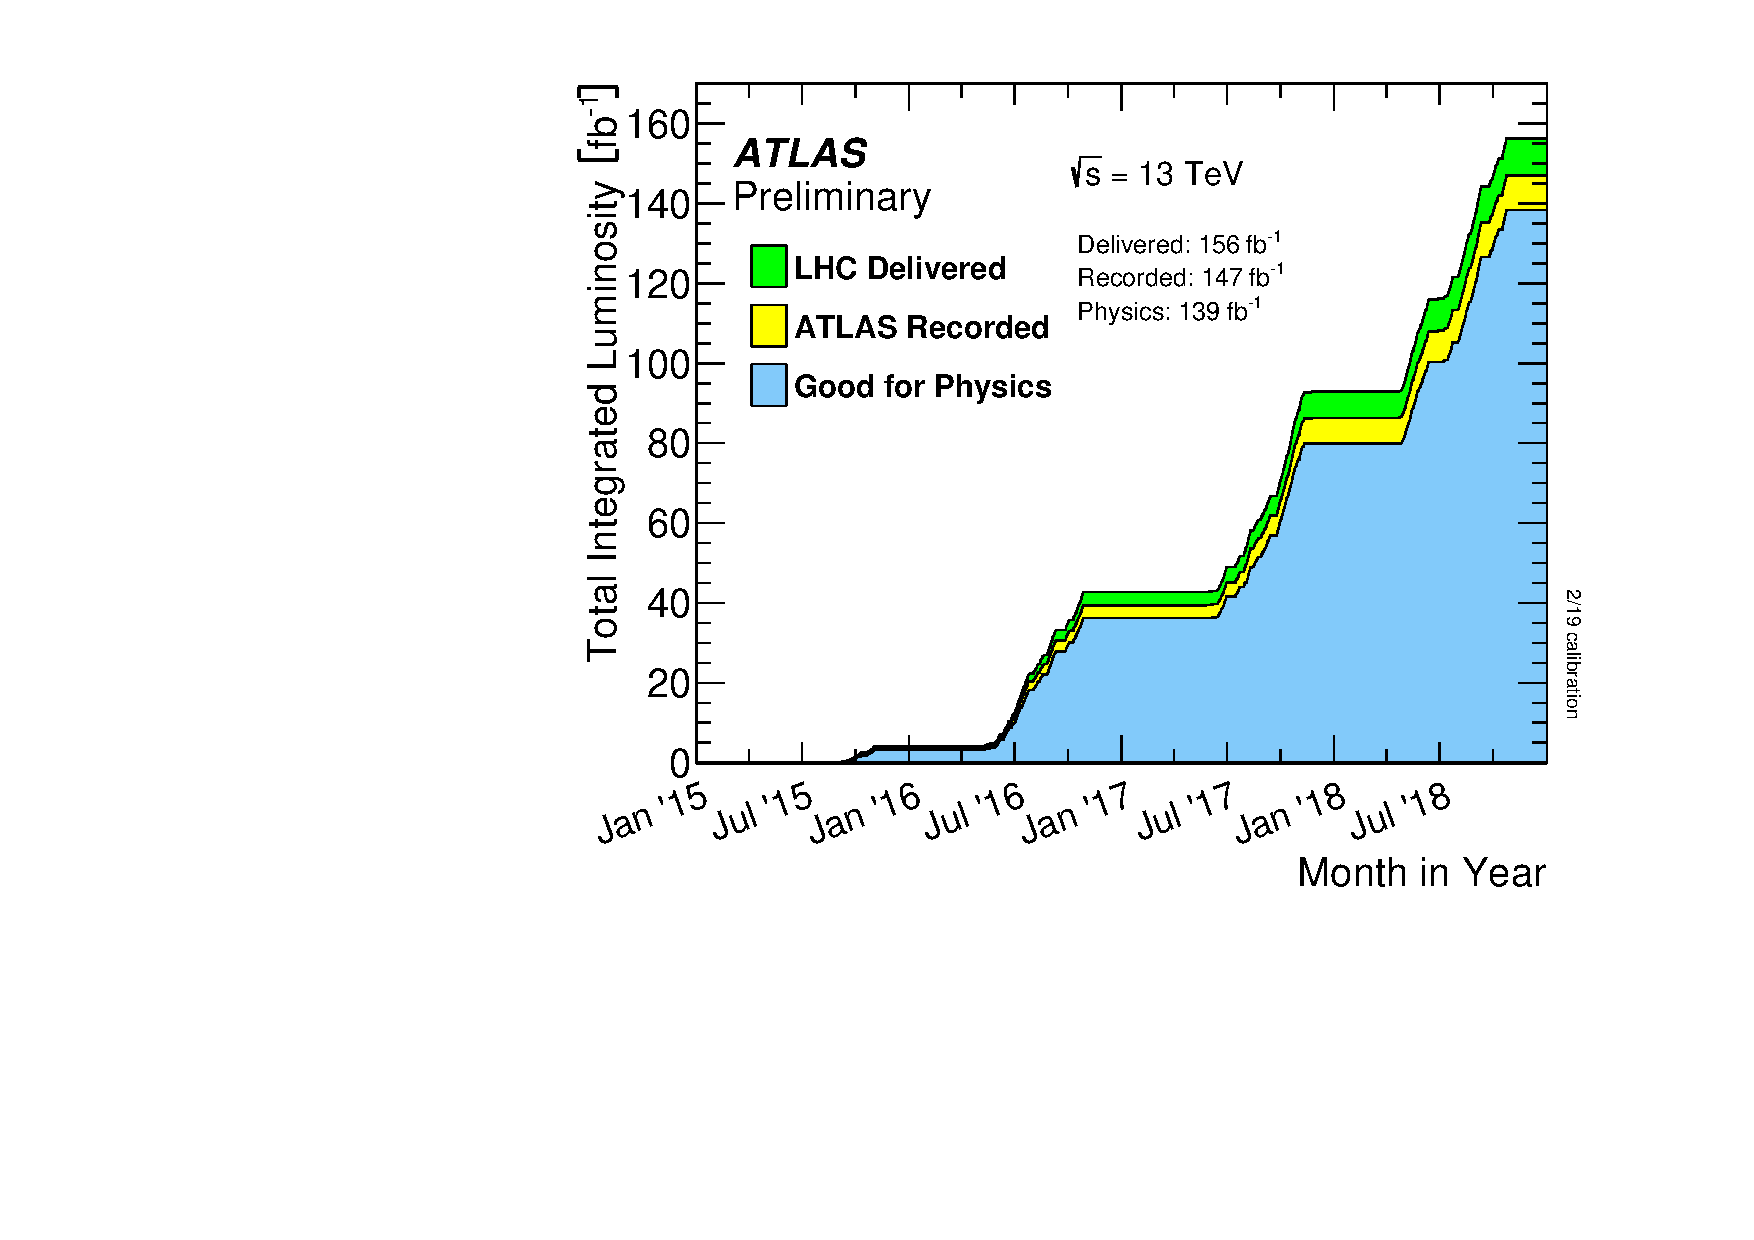
\includegraphics[width=0.45\textwidth,keepaspectratio]{figures/intlumivstimeRun2DQall.pdf}
\caption[f]{
Cumulative luminosity delivered to ATLAS (green), recorded by ATLAS (yellow), and good quality data (blue) during full Run~2 period.
}
\label{fig:luminosity}
\end{center}
\end{figure}

\subsection{Signal and Background Monte Carlo simulation}
\label{subsec:sigbgMC}
The details of the signal and the background modeling in the Monte-Carlo simulation are discussed in this subsection.
The Monte Carlo (MC) samples are used for the modelling of the background process, optimization of the event selection and the multivariate techniques for enhancing the signal sensitivities, and the estimation of systematic uncertainties.
\\ \\
\noindent\textbf{\sf{Signal EW VV+jj process}} \\ 
The EWK VV+jj production signal is modeled using MadGraph5\_aMC@NLO v2.3.3~\cite{Alwall:2014hca} event generator, with PYTHIA8~\cite{Sjostrand:2007gs} for the parton shower modeling and hadronization. The \textsc{NNPDF30LO} PDF set~\cite{Ball:2012cx} is used. 
The EWK VV+jj\ samples are generated at LO with two on-shell $V$ bosons, with one $V$ boson decaying leptonically
($Z\to \ell\ell$ with $\ell = e, \mu$, $Z\to \nu\nu$, $W\to \ell \nu$ with $\ell= e, \mu, \tau$),
and the other $V$ boson decaying hadronically. For the $W$ boson, both $W^{+}$ and $W^{-}$ are considered.
For each sample, all of the purely-electroweak tree-level diagrams (i.e. $\mathcal{O}(\alpha_{EW}^6)$ diagrams) that contribute to the final state are considered.

%The signal samples are generated with two on-shell V bosons (V is Z or W), one of which decays leptonically, and the other hadronically (semi-leptonic final states).
%Theoretically, VBS processes shown in Fig~\ref{fig:feynmanVBS} cannot be distinguished from the other electroweak VV+jj proceses like diagrams shown in Fig~\ref{fig:feynmanEWKnonVBS2} and Fig~\ref{fig:feynmantZb}, for the gauge invariant conservation, hence they are generated altogether as electroweak (EW) VV+jj production.

%% feynman diagrams, VBS
%\begin{figure}[H]
%\begin{center}
% 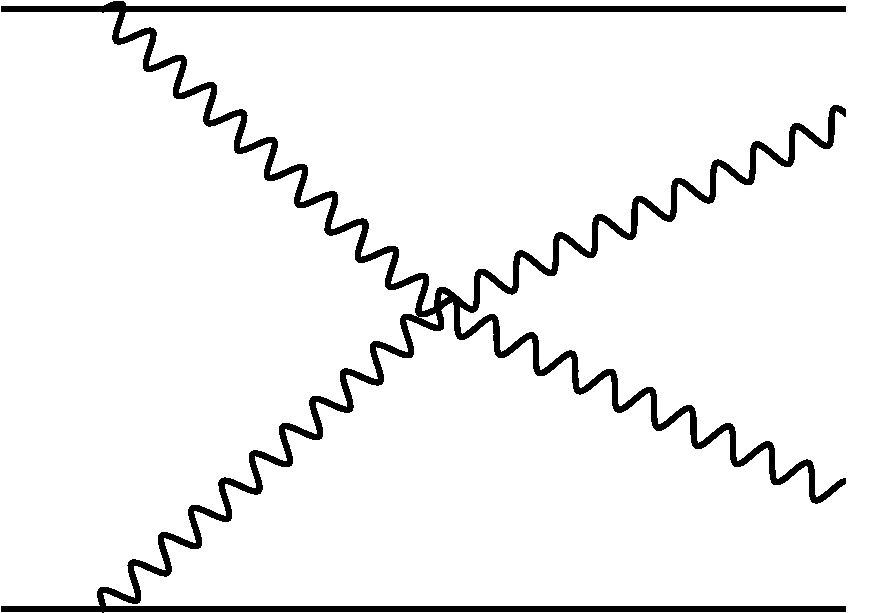
\includegraphics[width=0.3\textwidth,keepaspectratio]{figures/samples/feynVBS2.pdf}
% 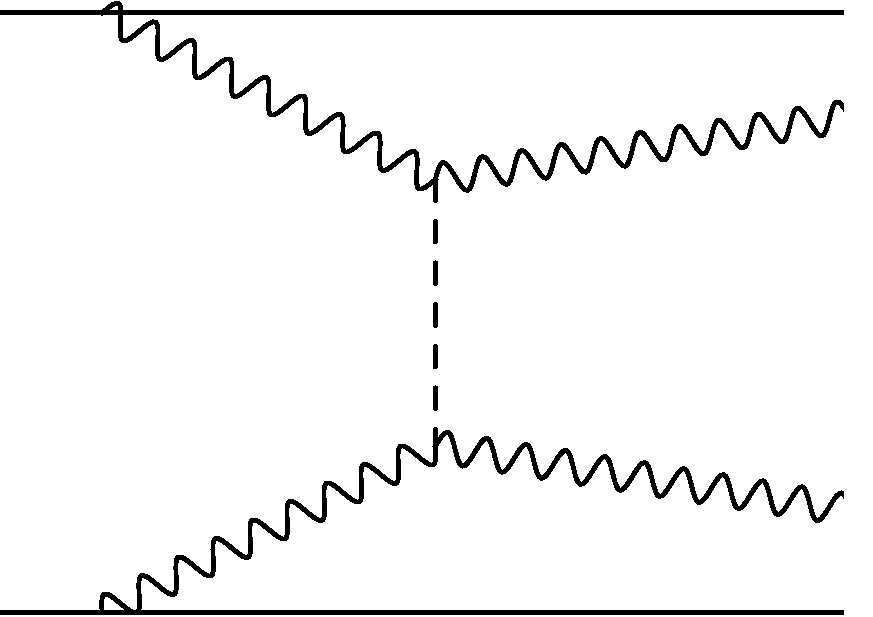
\includegraphics[width=0.3\textwidth,keepaspectratio]{figures/samples/feynVBS1.pdf}
% 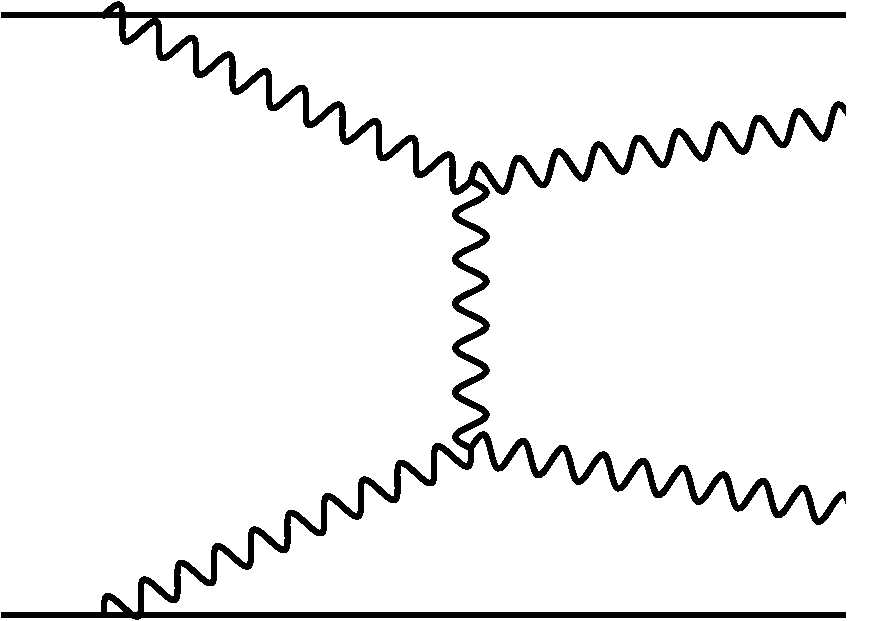
\includegraphics[width=0.3\textwidth,keepaspectratio]{figures/samples/feynVBS3.pdf}
% 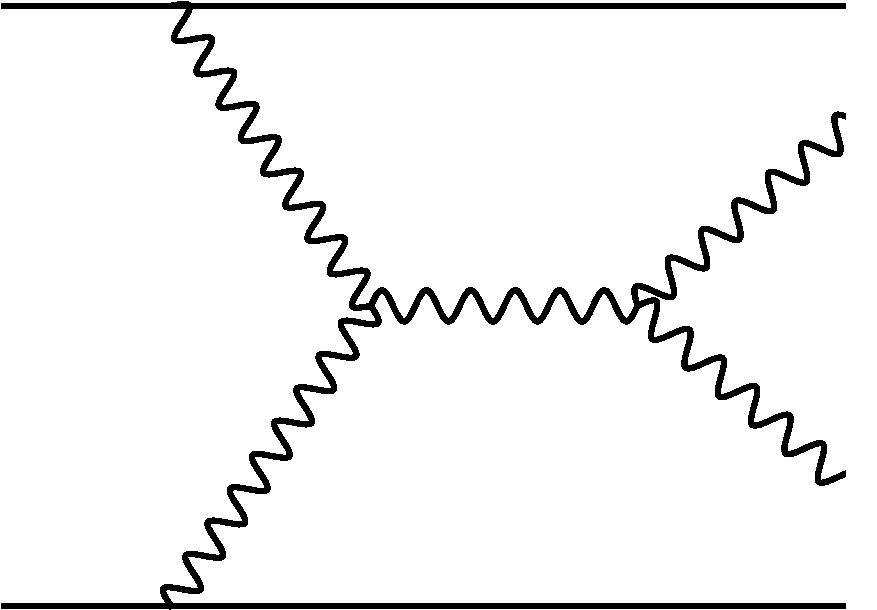
\includegraphics[width=0.3\textwidth,keepaspectratio]{figures/samples/feynVBS4.pdf}
% 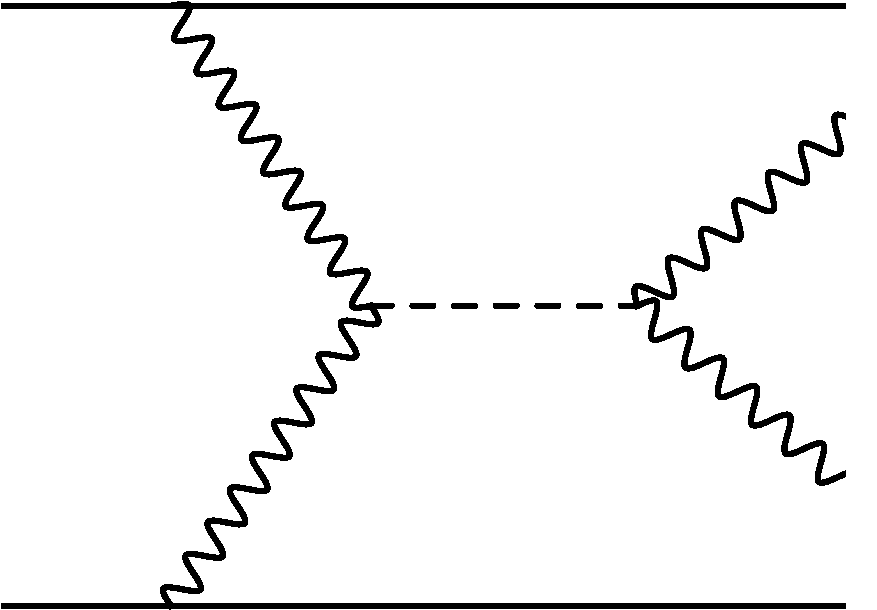
\includegraphics[width=0.3\textwidth,keepaspectratio]{figures/samples/feynVBS5.pdf}
%\caption[f]{
%VBS diagrams contribute to the signal.  
%The dashed line represents the Higgs boson.The decay products of the bosons are not shown.
%}
%\label{fig:feynmanVBS}
%\end{center}
%\end{figure}

%The non-VBS diagrams, which do not includes the boson scattering, shown in Figure~\ref{fig:feynmanEWKnonVBS1}, \ref{fig:feynmanEWKnonVBS2}. 

%% feynman diagrams, non-VBS
%\begin{figure}[H]
%\begin{center}
% 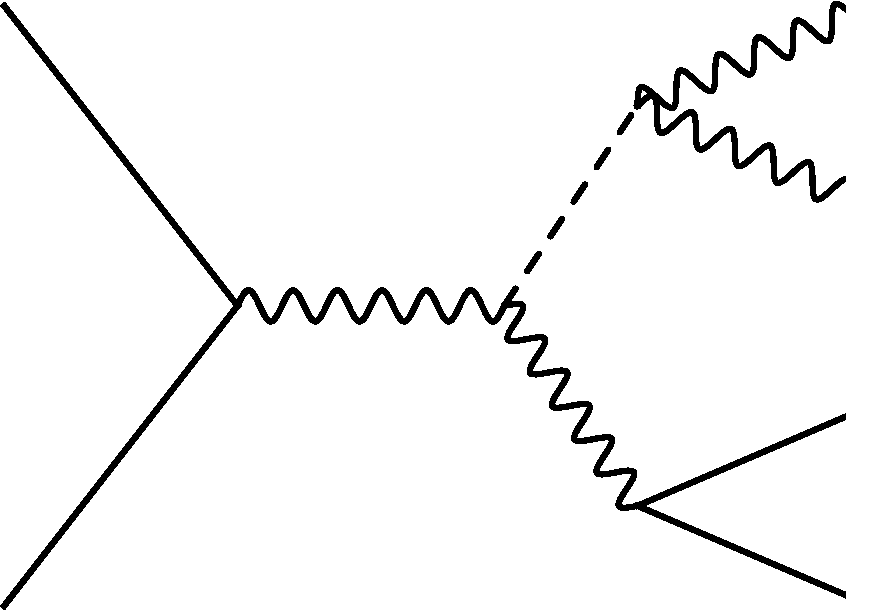
\includegraphics[width=0.30\textwidth,keepaspectratio]{figures/samples/feynEWKnonVBS3.pdf}
% 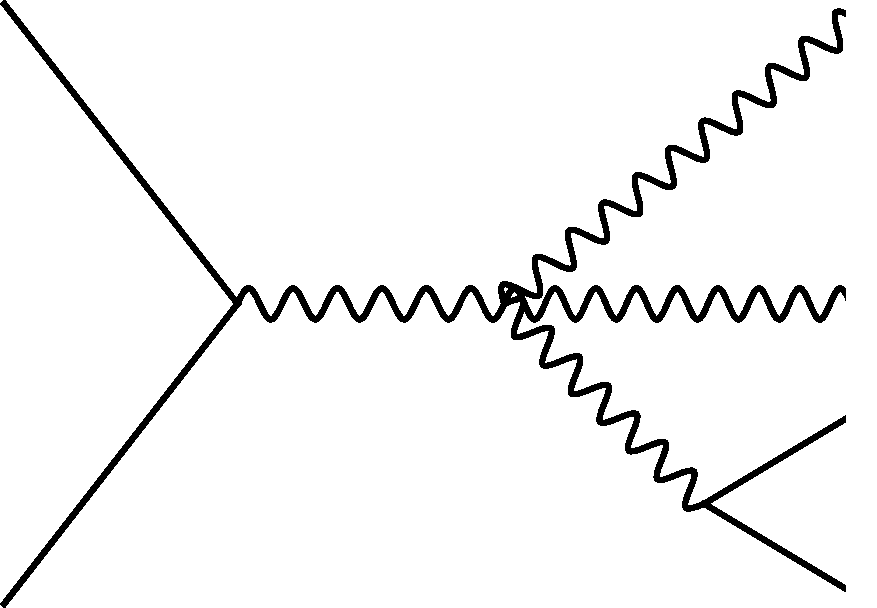
\includegraphics[width=0.30\textwidth,keepaspectratio]{figures/samples/feynEWKnonVBS4.pdf}\\
% 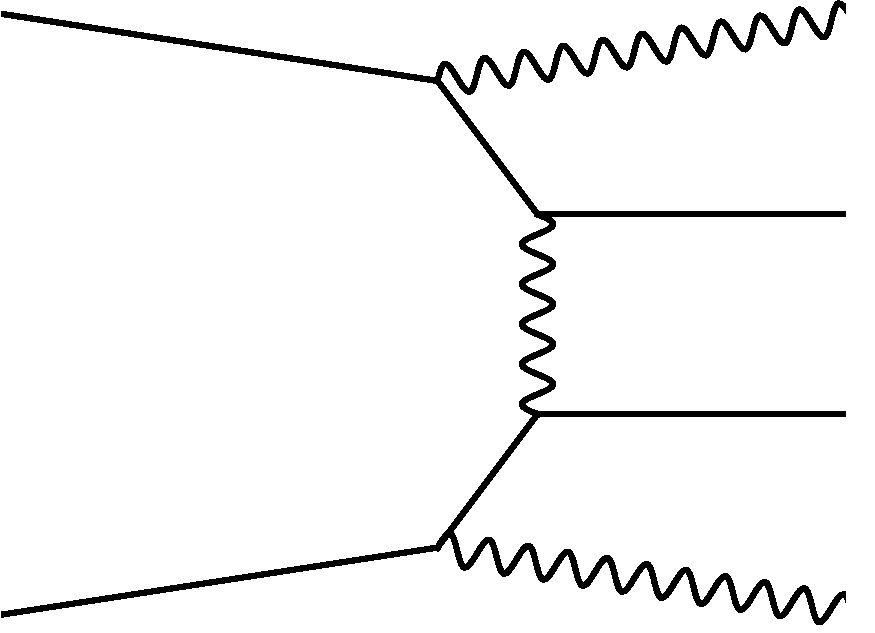
\includegraphics[width=0.30\textwidth,keepaspectratio]{figures/samples/feynEWKnonVBS5.pdf}
% 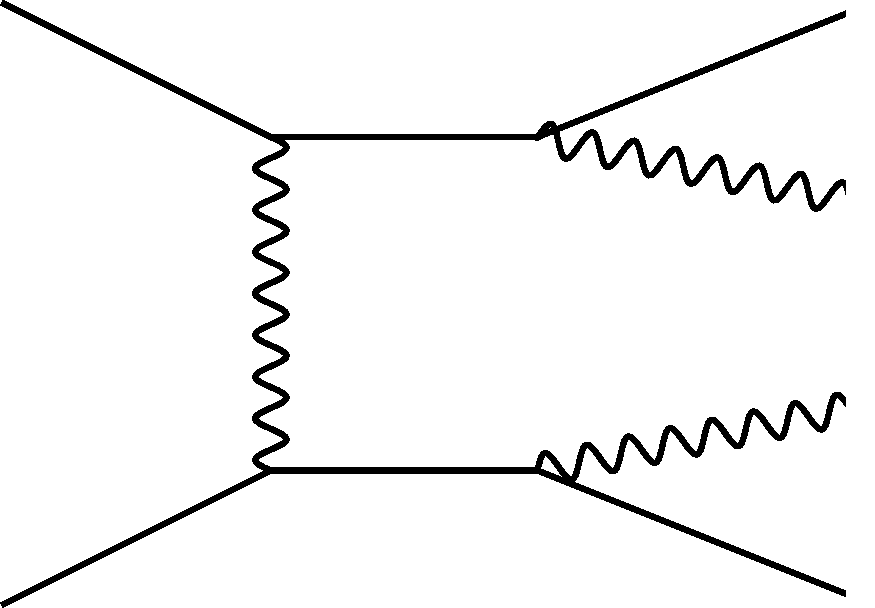
\includegraphics[width=0.30\textwidth,keepaspectratio]{figures/samples/feynEWKnonVBS6.pdf}
% \caption[f]{
%non-VBS diagrams contribute to the signal. 
%}
% \label{fig:feynmanEWKnonVBS1}
%\end{center}
%\end{figure}

\begin{figure}[H]
\begin{center}
 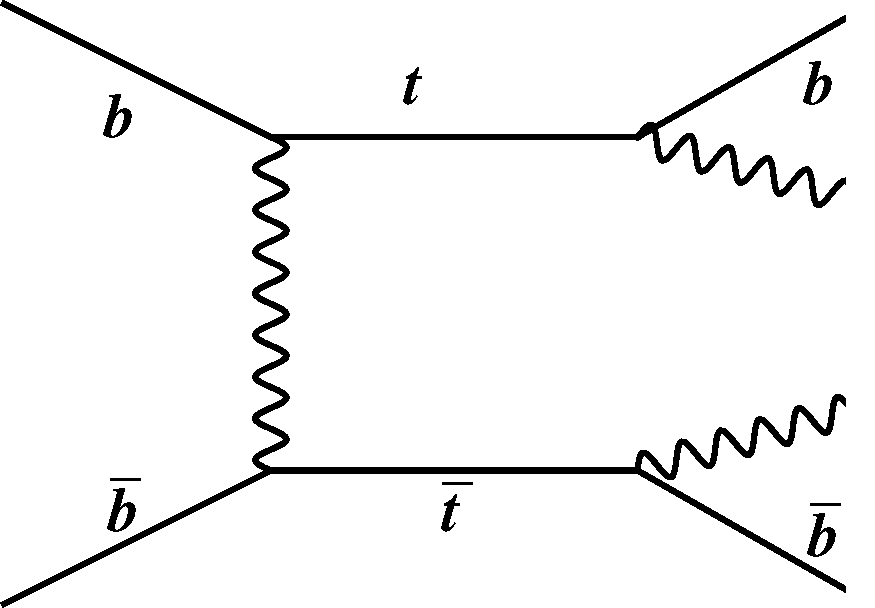
\includegraphics[width=0.25\textwidth,keepaspectratio]{figures/samples/feynEWKnonVBS1.pdf}
 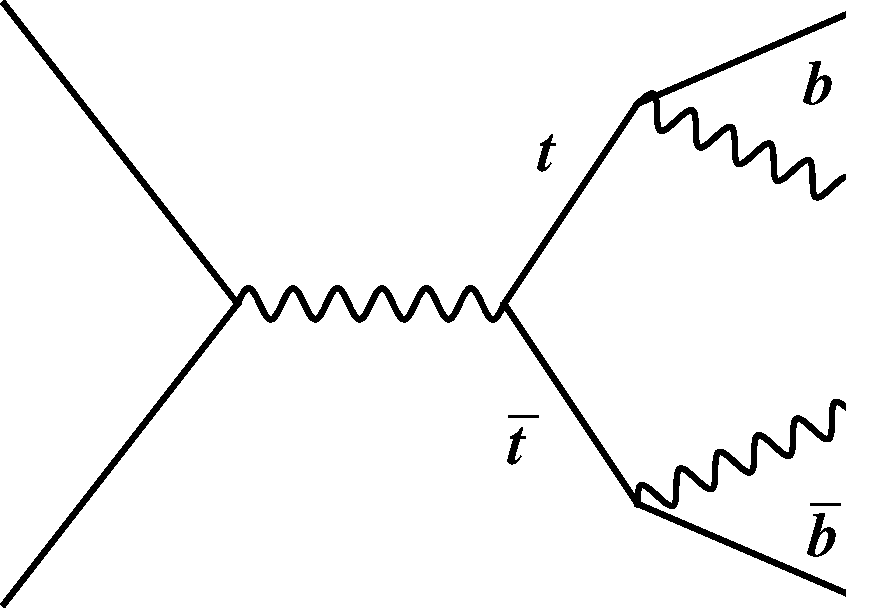
\includegraphics[width=0.25\textwidth,keepaspectratio]{figures/samples/feynEWKnonVBS2.pdf}
 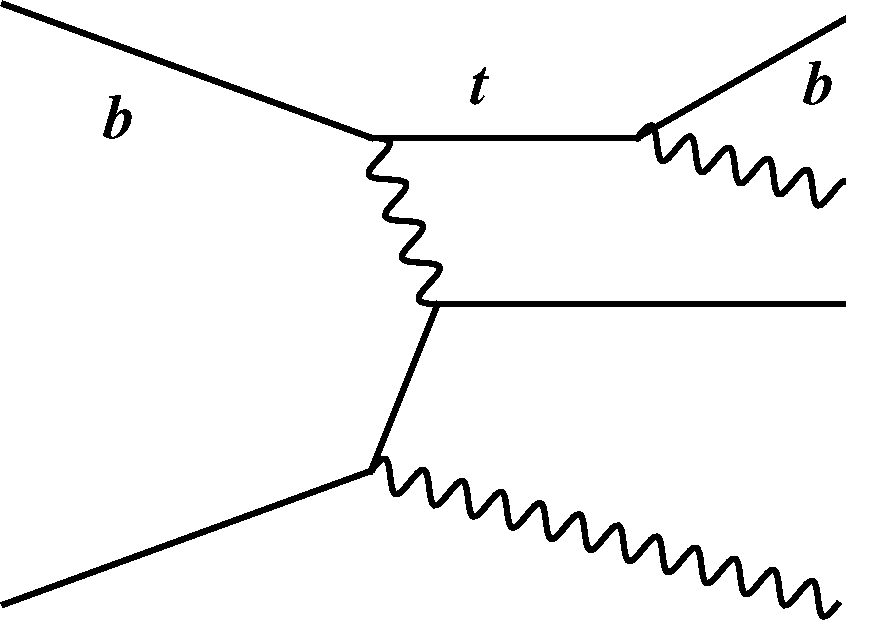
\includegraphics[width=0.25\textwidth,keepaspectratio]{figures/samples/feynEWKnonVBS7.pdf}
 \caption[f]{
non-VBS diagrams contribute to the signal, include top.
}
\label{fig:feynmanEWKnonVBS2}
\end{center}
\end{figure}

%% feynman diagram, tZb
\begin{figure}[H]
\begin{center}
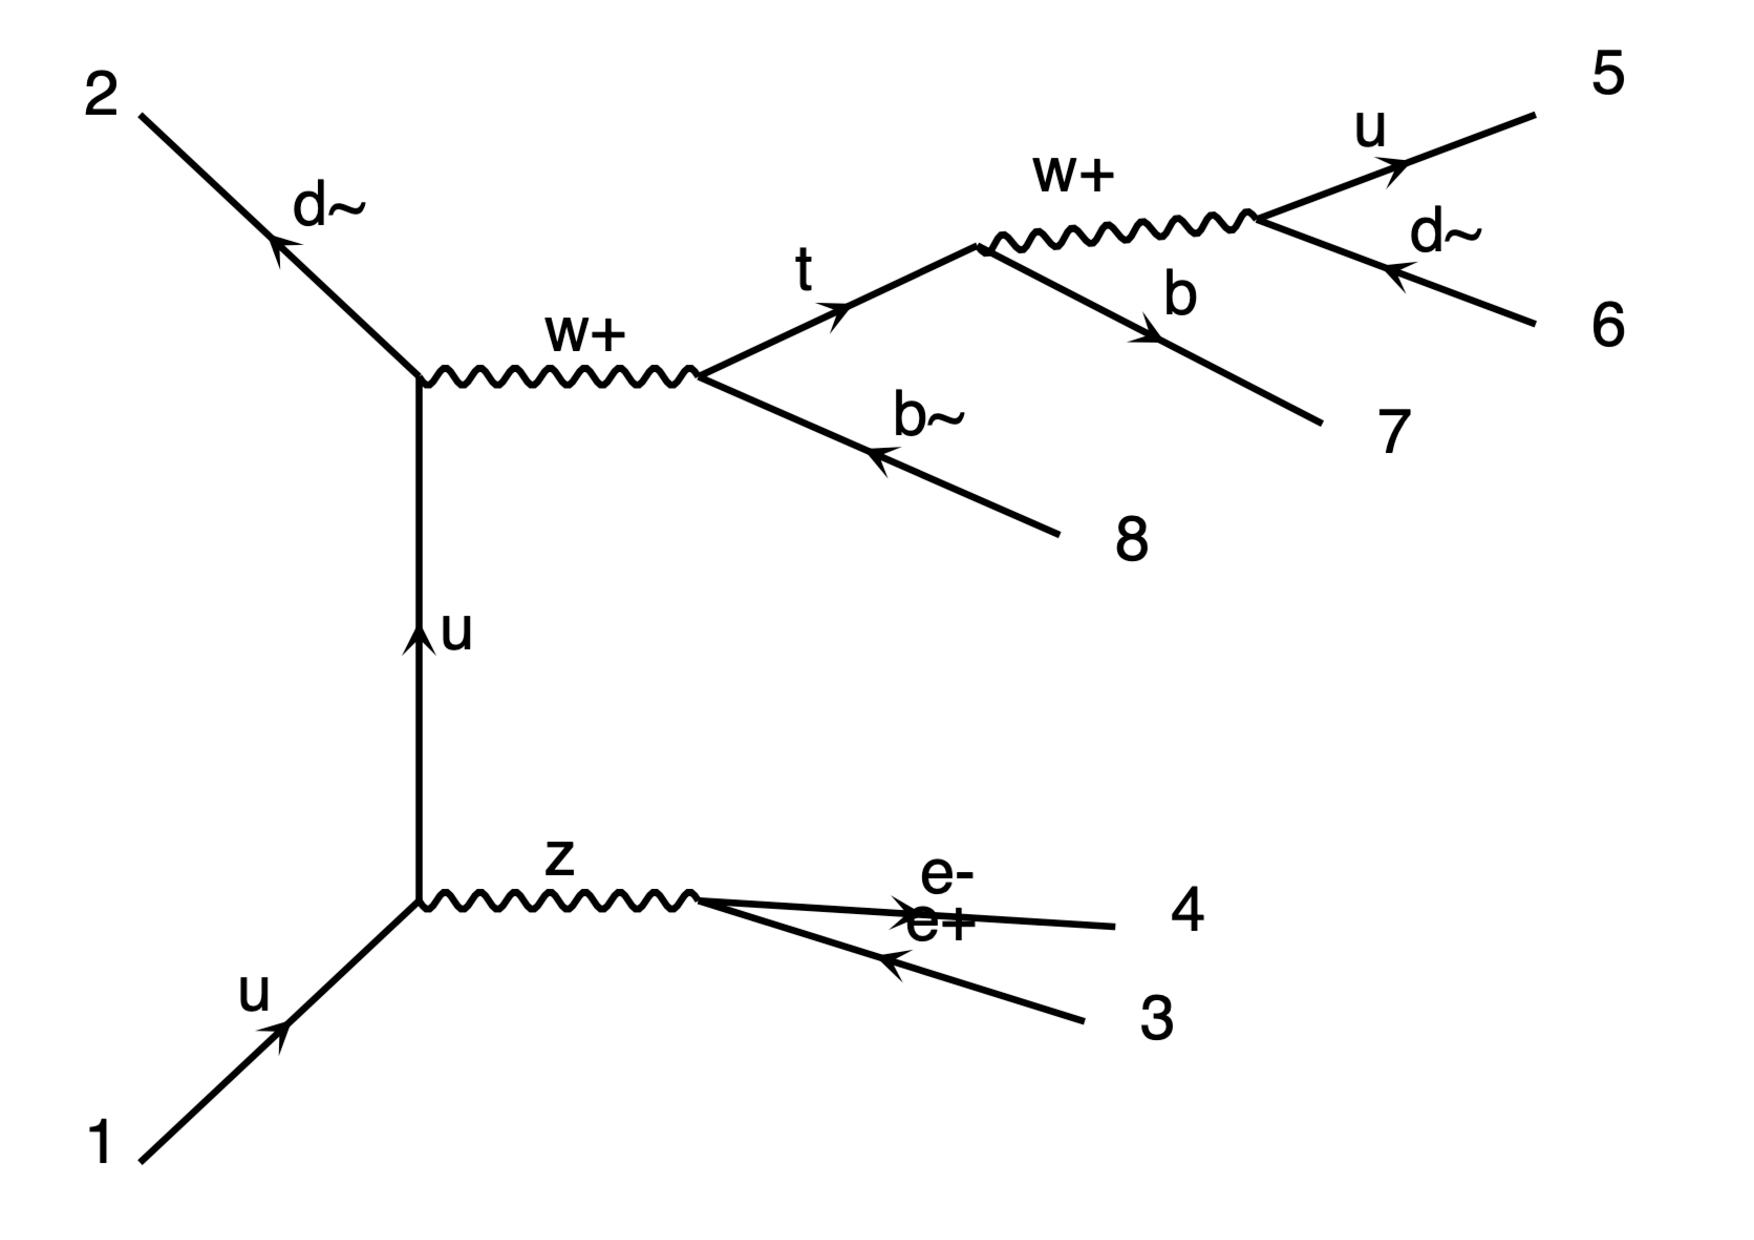
\includegraphics[width=0.4\textwidth,keepaspectratio]{figures/samples/feynEWKnonVBStZb.pdf}
\caption{
The example of the tZb diagram, which included in non-VBS diagrams.
}
\label{fig:feynmantZb}
\end{center}
\end{figure}

Especially the contribution from electroweak ttbar process shown in figure~\ref{fig:feynmanEWKnonVBS2} is included about 50~\% of the whole EW VV+jj signal samples, which can be suppressed by applying b-veto (not requiring the b-tagged jets). After applying b-veto in the event selection, there is still non-negligible contributions from tZb process, shown in figure~\ref{fig:feynmantZb}. This contributions are reduced by applying additional cut descibed in section~\ref{sec:eventselection}.
The production cross-section calculated by the MadGraph is shown in the table~\ref{tab:VBS_sig_samples}. \\ 
\begin{table}[!htbp]
\begin{center}
\small
\begin{tabular}{|l|l|}
\hline
Process & cross-section~(pb) \\
\hline
$W(l\nu)W(qq\prime)jj,b-veto$    &  1.99    \\
$W(l\nu)W(qq\prime)jj,b-filter$  &  1.97   \\
$W(l\nu)W(qq\prime)jj$            &  3.96   \\
$W(l\nu)Z(qq\prime)jj$            &  0.25   \\
$W(\nu\nu)W(qq\prime)jj$          &  0.15   \\
$Z(ll)W(qq\prime)jj$              &  0.045  \\
$Z(\nu\nu)Z(qq\prime)jj$          &  0.032  \\
$Z(ll)Z(qq\prime)jj$              &  0.0096 \\
\hline
\end{tabular}
\caption{List of production cross sections of the signal samples. b-veto/b-filter correspond to samples without/with decays containing $b$-quarks.}
\label{tab:VBS_sig_samples}
\end{center}
\end{table}

\noindent\textbf{\sf{Background processes}} \\ 
%The Background processes in this analysis includes  $W$/$Z$ $\plus$ jets, $t\bar{t}$, single top, diboson (WW,WZ,ZZ) and multi-jets production. 
%The main background for this analysis is the V($W$/$Z$)$\plus$ jets, which is the single W or Z boson in associated with jets. The final state is different with the EWVVjj signal though this is the dominant background process especially for 0-lepton and 2-lepton channel.
The $W$/$Z$ + jets background is modeled using Sherpa~2.2.1~\cite{Gleisberg:2008ta} generator. 
Matrix element is calculated for up to 2 partons at next-to-leading order (NLO), and 4 partons at leading order (LO) with Comix~\cite{Gleisberg:2008fv} and OpenLoops\cite{Cascioli:2011va} matrix element generators, with the Sherpa parton shower~\cite{Schumann:2007mg} using the ME+PS@NLO prescription~\cite{Hoeche:2012yf}.
The NNPDF3.0NNLO PDF set is used in association to authors' tuning. The resulting events are normalized to the NNLO cross sections.

The QCD diboson background is also generated with Sherpa~2.2.1 generator. 

%The $t\bar{t}$ proceess has the same final state as EWVVjj signal process, which has two jets include b-hadron, and two W bosons decay to the leptons and hadrons. This can be the large background in 1-lepton channel, and can be reduced by requiring not to have b-tagged jets. There are minor contributions from single-top process, which is also suppressed by b-vetoing.
Single-top and $t\bar{t}$ backgrounds are generated with the Powheg-Box~\cite{Alioli:2010xd} generator with the NNPDF3.0NLO PDF\cite{Ball:2014uwa} sets in the matrix element calculation. The top mass is set to $172.5~\mathrm{GeV}$. The parton shower and the hadronization is simulated using \textsc{Pythia}~8.230. \\
%The top quark spin correlations are preserved (for t-channel, top quarks are decayed using MadSpin~\cite{Artoisenet:2012st}). For all processes the parton shower, fragmentation, and the underlying event are simulated using \textsc{Pythia}8.230 with the A14 tune set\cite{ATL-PHYS-PUB-2014-021}. The top mass is set to $172.5\gev$. The cross sections of $t\bar{t}$ and single-top are known to NNLO in QCD including re-summation of next-to-next-to-leading logarithmic (NNLL) soft gluon terms\cite{Czakon:2011xx,Kidonakis:2011wy,Kidonakis:2010tc,Kidonakis:2010ux}.
%The parameter \textsc{Hdamp} to regulate the high-\pt\ radiation in the \textsc{Powheg} is set to $1.5m_{t}$ for a good data/MC agreement at high \pt\ region\cite{ATL-PHYS-PUB-2016-020}.
%The diboson processes ($WW$, $WZ$ and $ZZ$) also have the same final states with the EWVVjj signals. They are generated with Sherpa 2.2.1~\cite{Gleisberg:2008ta} generator.

All simulated events are processed with the same trigger and reconstruction algorithm as the data.
Additional $pp$ collisions generated with \textsc{Pythia}~8.186\cite{Sjostrand:2008vc} are overlaid to model the effect of the pileup, the particles coming from secondary collisions in the same data-taking timing, for all MC events.
In order to take into account the detector geometry and the reconstruction efficiency, samples are processed through the full ATLAS detector simulation\cite{SOFT-2010-01} based on \textsc{GEANT4}\cite{Agostinelli:2002hh}.

\subsection{aQGC signal process Monte Carlo simulation}
To model possible aQGC effect in the VBS process, the Eboli model \cite{eboli2006p} which introduces 21 new dim-8 operators is used as described in section~\ref{subsec:EFT}.
Of these operators, 19 can effect the semileptonic VBS final state.
%As typical for EFT expansions, the modified lagrangian with these new operators $\mathcal{L}_n$ and corresponding Wilson coeffiencts $c_n$ and UV scale $\Lambda$ is:
%\begin{equation*}
%  \mathcal{L}=\mathcal{L}_{sm}+\sum_{n}\frac{c_n}{\Lambda^{4}}\mathcal{L}_n
%\end{equation*}

In generality, the matrix-element of a SM process with the addition of new EFT contributions can be written as:
\begin{equation}
  |A_{SM}+c_iA_i|=|A_{SM}|^2+\sum\limits_i c_i^2|A_{i}|^2+ \sum\limits_i 2 c_i \mathrm{Re}(A_{SM}^\star A_i) +\sum\limits_{i\neq j} c_i c_j \mathrm{Re}(A_i^\star A_j)
\end{equation}
where $|A_{SM}|^2$ is the SM matrix element, $|A_{i}|^2$ represents the pure-EFT matrix element, $2 \mathrm{Re}(A_{SM}^\star A_i)$ is their corresponding interference term, and $\mathrm{Re}(A_i^\star A_j)$ is the possible interference between EFT amplitudes.
This structure can be exploited in recent MadGraph5\_aMC@NLO versions which allows the specific generation of each of these terms individually, known as the matrix-element decomposition method.

Typically one would need to generate a series of samples for each operator $A_i$ at different $c_i$ values, to derive a series of template functions for $|A_{SM}+c_iA_i|$ which would need to be interpolated between for arbitrary $c_i$. Generating samples with the decomposition method greatly simplifies this procedure as one only now needs to generate for each operator $A_i$ the corresponding pure-EFT and interference terms (as well as cross-interference terms if needed). These templates can then be scaled either quadratically or linear with the corresponding $c_i$ values to generate the required full template $|A_{SM}+c_iA_i|$.

The Eboli dim-8 EFT processes are modeled using MadGraph5\_aMC@NLO v2.7.2~\cite{Alwall:2014hca} at LO with the \textsc{NNPDF30LO} PDF set~\cite{Ball:2012cx} plus \PYTHIA8.244~\cite{Sjostrand:2007gs} for fragmentation.
The matrix-element calculation produces two on-shell $W/Z$ bosons, which are subsequently decayed with \textsc{Madspin}~\cite{Artoisenet:2012st} to simulate the leptonic and hadronic decays of the bosons.
The use of Madspin is required for use of the matrix-element weighting and requires separate generation for each weak isospin state of the boson (i.e the following processes are simulated separately: $W^+W^-$, $W^+W^+$, $W^-W^-$, $W^+Z$, $W^-Z$, $ZZ$). \\ \\


%\subsection{Data sets}

%\begin{table}[htb!p]
%\caption{An integrated luminosity used in this analysis. }
%\label{tab:intLumi}
%\begin{center}
%\begin{tabular}{|l|l|}
%\hline
%Year & $\mathcal{L}$ [fb$^{-1}$] \\
%\hline\hline
%2015 & 3.21 \\
%\hline
%2016 & 32.88 \\
%\hline
%2017 & 44.31 \\
%\hline
%2018 & 59.94 (21) for $\ell\nu qq$/$\ell\ell qq$ ($\nu\nu qq$) channel \\
     %& (will be updated to 58.45 with the latest lumi-tag) \\
%2018 & 58.45 \\
%\hline\hline
%total & $139.0 \pm 2.4$ \\
%\hline
%\end{tabular}
%\end{center}
%\caption{An integrated luminosity used in this analysis. }
%\end{table}





